% Leetcode 208. Implement Trie (Prefix Tree)
\noindent \textred{4.} 
(\textbf{Radix trees}) Given two strings, $a = a_0 a_1 a_2 \dots a_p$ and $b = b_0 b_1 b_2 \dots b_q$, where each $a_i$ and each $b_j$ belongs to some ordered set of characters, we say that string $a$ is \textit{lexicographically} less than string $b$ if either 
\begin{enumerate}
    \item[i] there exists an integer $j$, where $0 \leq j \leq \min\{p, q\}$, such that $a_i = b_i$ for all $i = 0, 1, \dots , j - 1$ and $a_j < b_j$ , or
    \item[ii] $p < q$ and $a_i = b_i$ for all $i = 0, 1, 2, . . . p$.
\end{enumerate}
For example, if $a$ and $b$ are bit strings, we can verify that $10100 < 10110$ and $10100 < 101000$ following the above rules. This ordering is similar to that used in English-language dictionaries. \\
The \textit{radix tree} data structure shown in Figure 12.5 (a.k.a. \textit{trie}) stores the bit strings 1011, 10, 011, 100
and 0. When searching for a key $a = a_0 a_1 a_2 \dots a_p$, go left at a node of depth $i$ if $a_i = 0$ and right if $a_i = 1$.
\begin{figure}[!h]
    \centering
    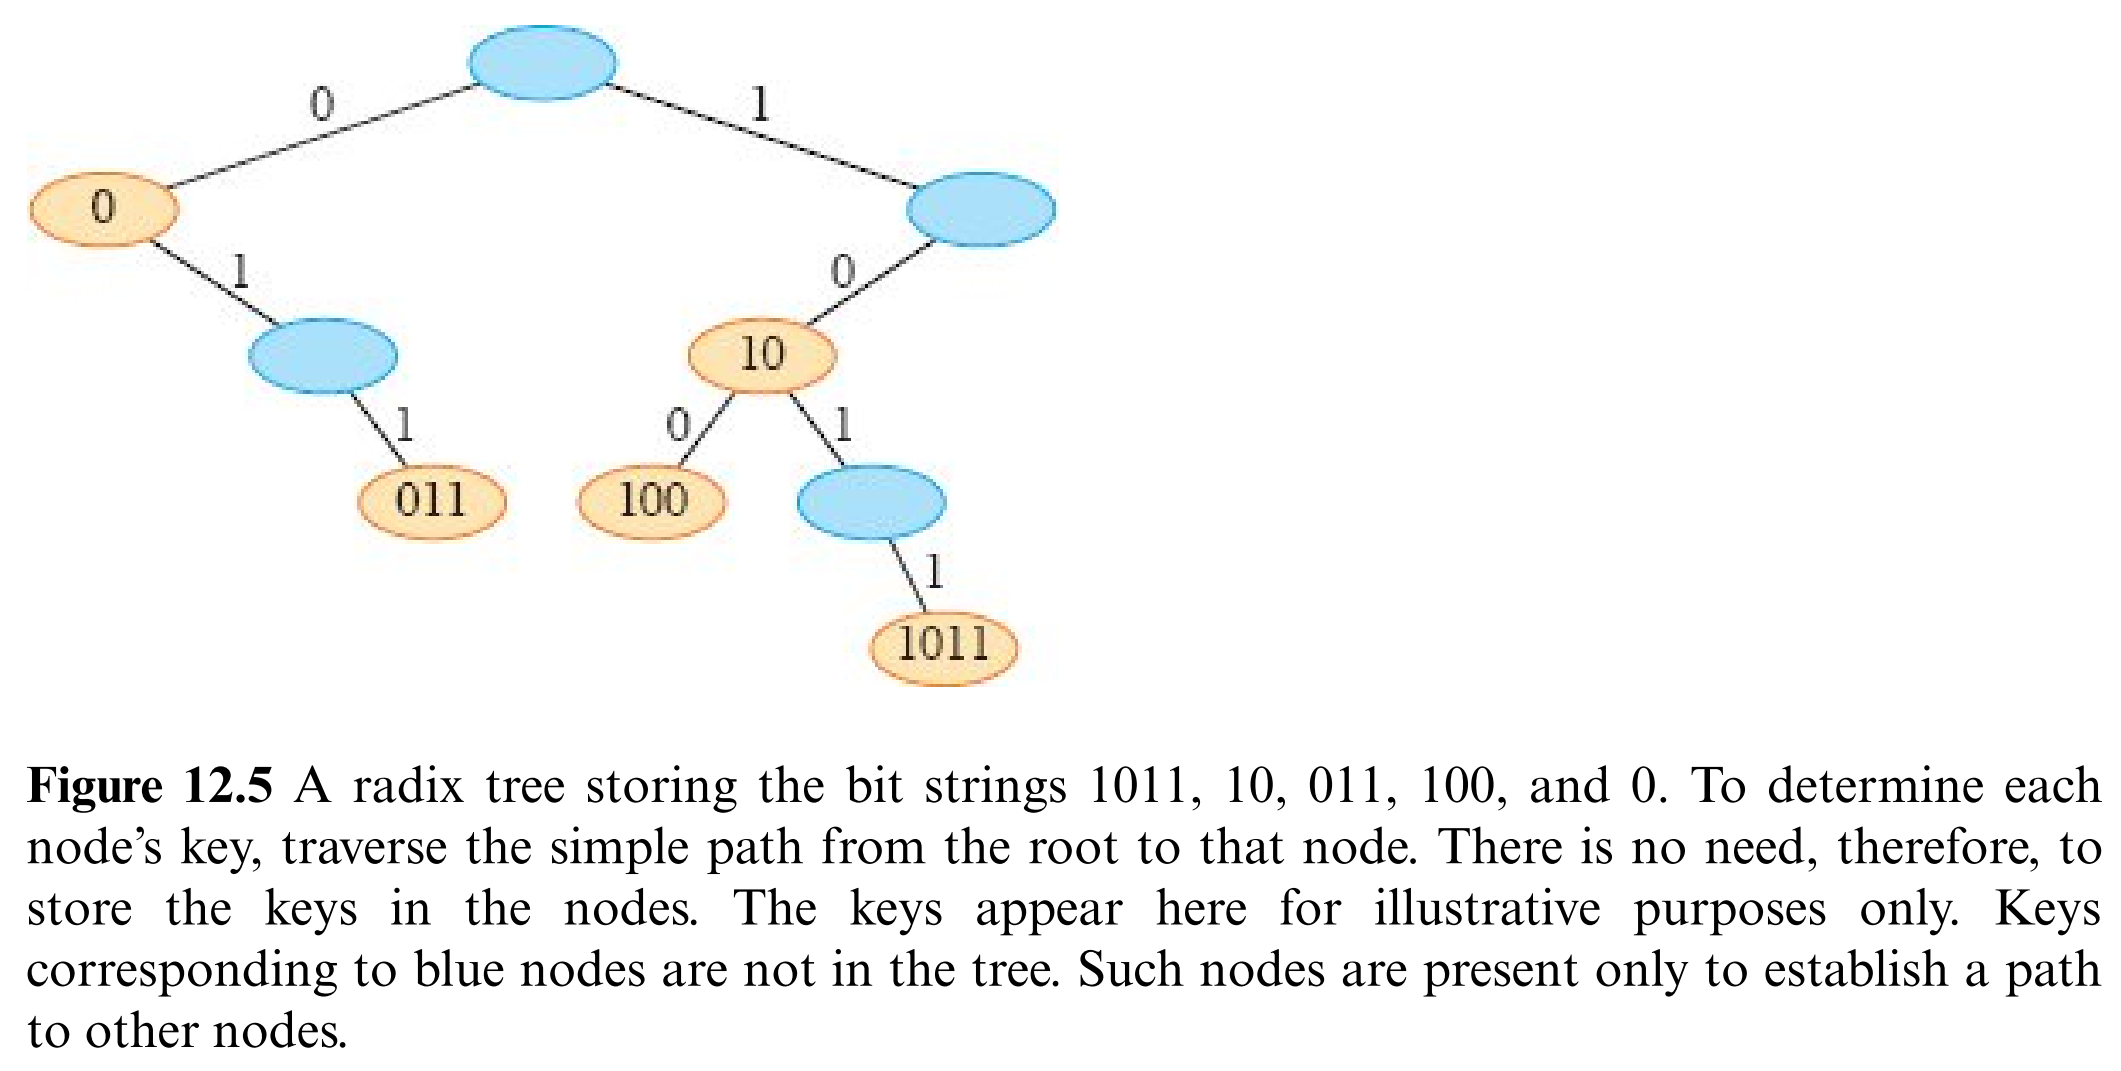
\includegraphics[width=\linewidth]{HWs//HW7//figures/4.png}
\end{figure}
\begin{itemize}
    \item[(a)] Let $S$ be a set of distinct bit strings whose lengths \textbf{sum to} $n$. Show how to use a radix tree to sort $S$ lexicographically in $\Theta(n)$ time. \\
    \myAnswer{
    Let lengths of bit strings in $S$ be $\{ l_1, l_2, \dots, l_m\}$, such that $\sum_{i=1}^m l_i = n$. While inserting the $i^{th}$ bit string into the radix tree, it costs $\Theta(l_i)$ because we need to trace from the root to the corresponding node according to every digit. Therefore, in total it costs $\sum_{i=1}^m \Theta(l_i) = \Theta(n)$ to build the complete radix tree. Then we can readily use pre-order traversal to print out the sorted $S$.
    }
    \item[(b)] Now consider that the ordered set of characters have a size of $k > 2$ (for lower-case alphabetic letters, $k = 26$). Let $S$ be a set of distinct strings whose lengths sum to $n$. Will lexicographically sorting still cost $\Theta(n)$ time? Why, or why not? \\
    \myAnswer{
    Yes, it will still cost $\Theta(n)$ because the only difference between binary bits and alphabetic letters is the number, which only influences the 
    maximum children number of each node.}
\end{itemize}
